\documentclass[tikz,border=5mm]{standalone}
\begin{document}
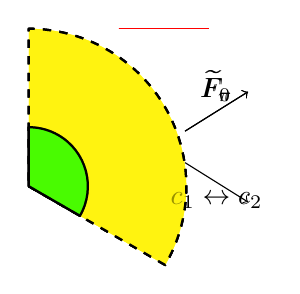
\begin{tikzpicture}[line join=round]
\def\Ang{-30}
\begin{scope}[local bounding box=L]
\draw[thick,dashed,fill=yellow,fill opacity=.6] 
(0,0) coordinate(O) -- ++(\Ang:2cm) coordinate(A) arc[radius=2cm,start angle=\Ang,end angle=90]
-- cycle;
\draw[thick,fill=green,fill opacity=.6] (O)--++(\Ang:.75cm) 
arc[start angle=\Ang,end angle=90,radius=.75cm] --cycle;
\end{scope}
\draw[red] (L.north)--(L.north east);
\begin{scope}[shift={(4,1)},local bounding box=R]
\draw[thick,dashed,fill=yellow,fill opacity=.6] 
(O)--++(\Ang:2cm) coordinate(A) arc[radius=2cm,start angle=\Ang,end angle=90]
-- cycle;
\draw[thick,fill=green,fill opacity=.6] (O)--++(\Ang:.75cm)
arc[start angle=\Ang,end angle=90,radius=.75cm] --cycle;
\end{scope}
\draw[red] (R.north)--(R.north east);
\draw[->] ([xshift=-3mm,yshift=2mm]L.east)--++(.8,.5) node[midway,above]{$\widetilde{F}_{0}$};
\draw[->] ([xshift=-3mm,yshift=-2mm]L.east)--++(.8,-.5) node[midway,below]{$c_{1}\leftrightarrow c_{2}$};
\begin{scope}[shift={(5,-3)},local bounding box=U]
\draw[thick,dashed,fill=yellow,fill opacity=.6] 
(O)--++(\Ang:2cm) coordinate(A) arc[radius=2cm,start angle=\Ang,end angle=90]
-- cycle;
\draw[thick,fill=green,fill opacity=.6] (O)--++(\Ang:.75cm)
arc[start angle=\Ang,end angle=90,radius=.75cm] --cycle;
\end{scope}
\draw[red] (U.north)--(U.north east);
\draw[->] ([xshift=-3mm,yshift=2mm]U.east)--++(.8,.5) node[midway,above]{$\widetilde{F}_{\pi}$};
\end{tikzpicture}
\end{document}